\begin{frame}\frametitle{Strategy}
\centering\myskip

\begin{minipage}{.25\textwidth}\centering
\footnotesize

$$\TTbar\to WbWb$$ 
like $$\ttbar\to WbWb$$

\myskip
\myskip


\includegraphics[width=1.15\textwidth]{pics/feyn_wbwb}


\end{minipage}\begin{minipage}{.75\textwidth}\centering
\vskip-5ex
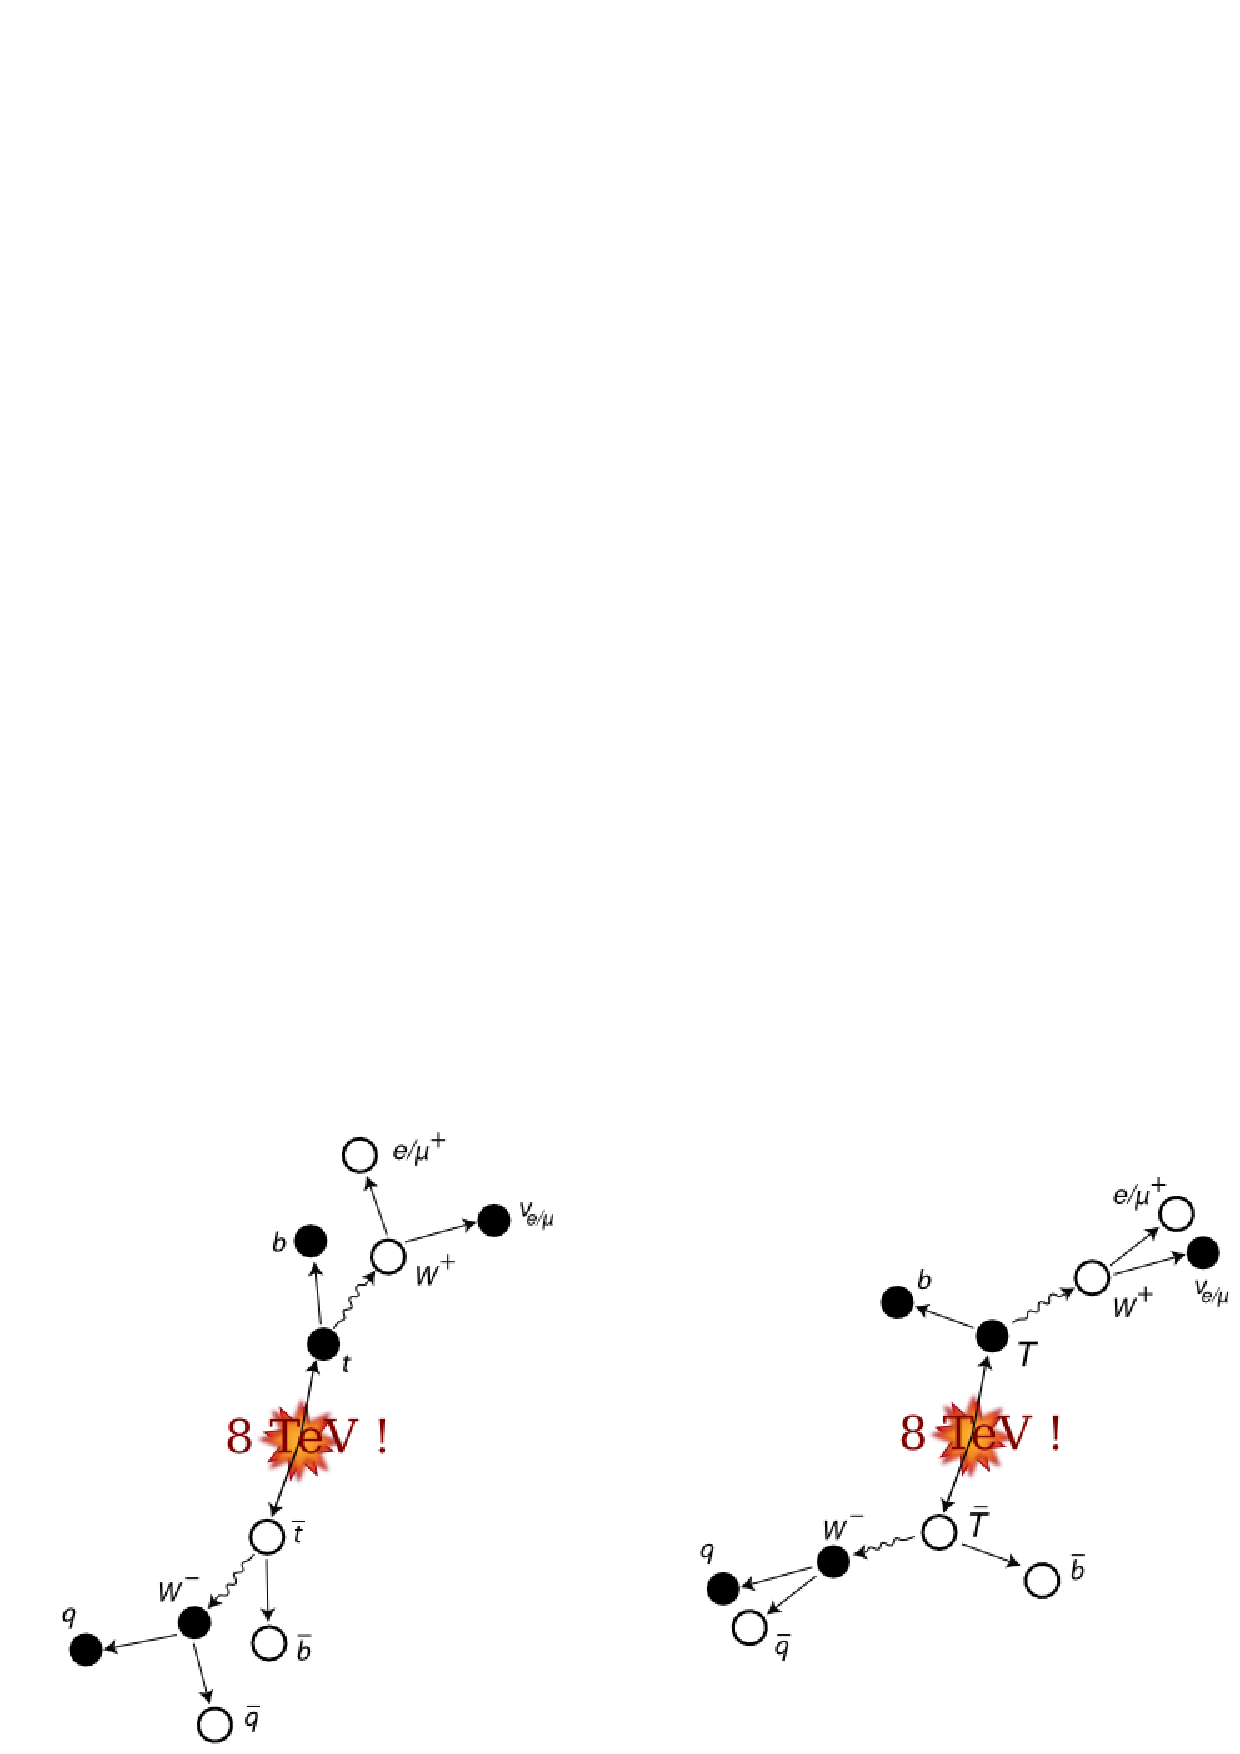
\includegraphics[width=1.\textwidth]{../wbx_analysis_14ifb/figures/kin.png}

different {\cccolor boosted kinematics}\\
{\LARGE $\Downarrow$}\\
reconstruct the $W$ boson from hadronic decay\\
{\LARGE $\Downarrow$}\\
reconstruct heavy quark mass

%{\LARGE $\swarrow\searrow$}\\
%\begin{minipage}{.3\textwidth}\centering
%merged jets\\
%\wi
%\end{minipage}\begin{minipage}{.3\textwidth}\centering
%close-by jets\\
%\wii
%\end{minipage}

\end{minipage}

\end{frame}

%%%%%%%%%%%%%%%%%%%%%%%%%
%%%
%%%%%%%%%%%%%%%%%%%%%%%%%
\begin{frame}\frametitle{$W$ boson reconstruction}
\centering\footnotesize

\begin{minipage}{.34\textwidth}\centering

{\cccolor \large \wi}

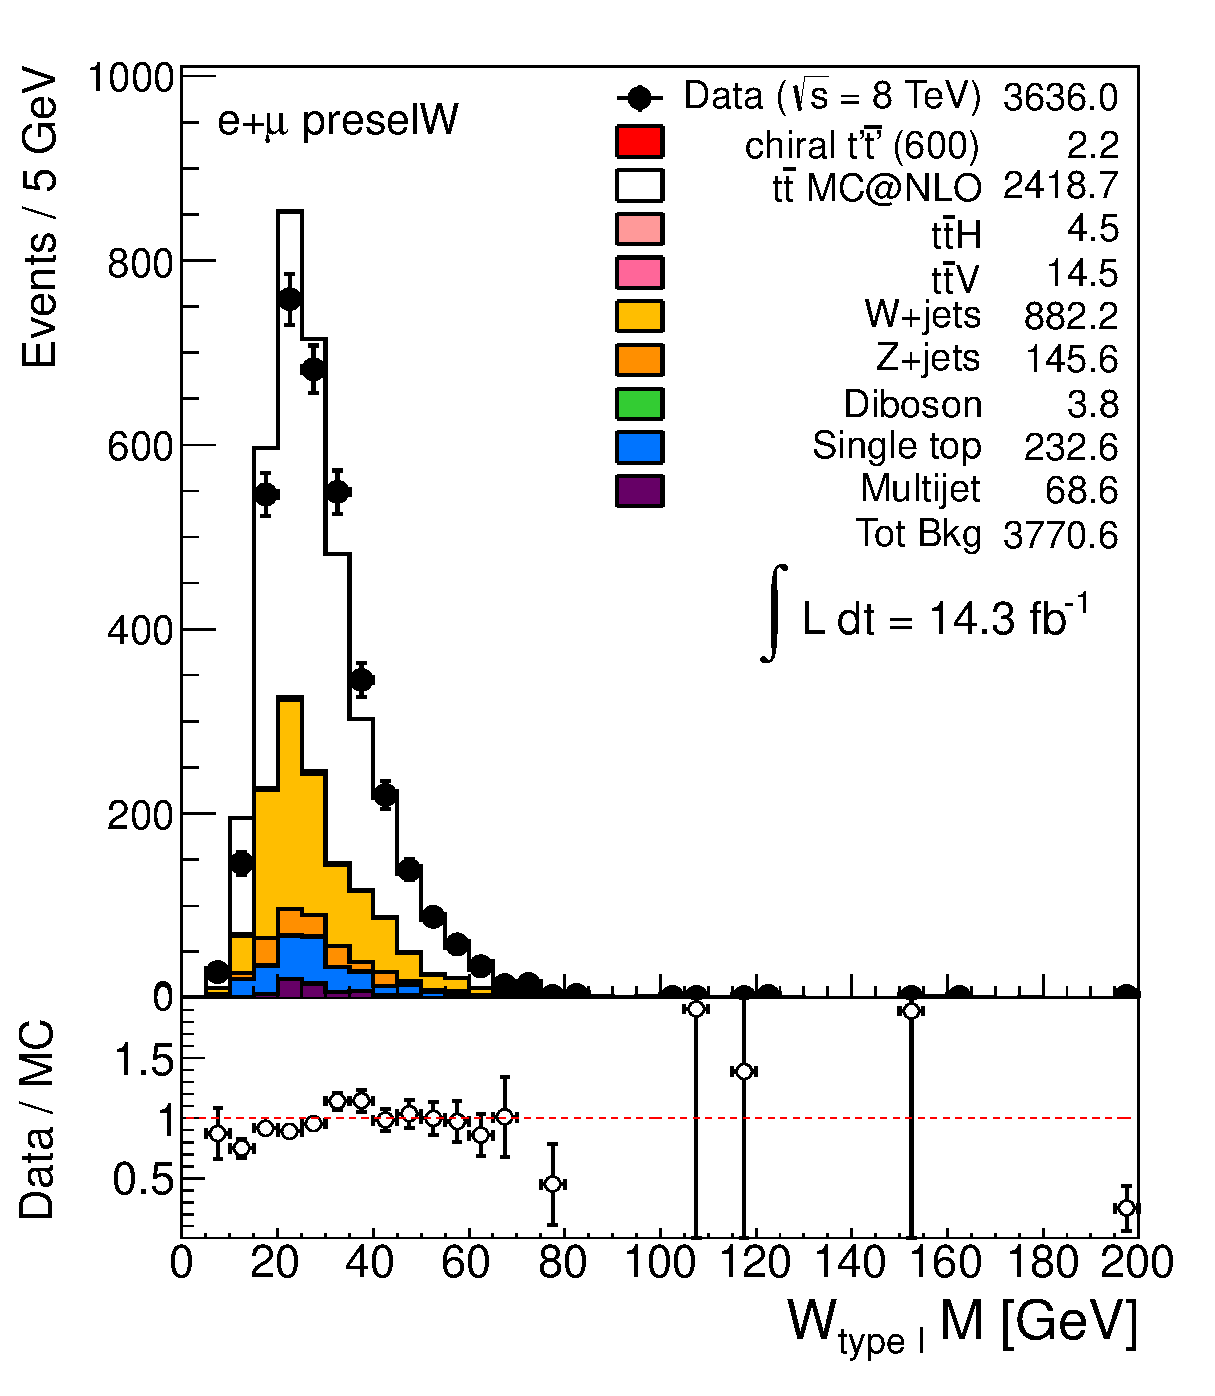
\includegraphics[width=1.\textwidth]{pics/VLQAna_WbX_WpreselType1_M_ELEMUON_preselW_NOMINAL}

\begin{pgfpicture}{0.0\textwidth}{0.0\textheight}{1.\textwidth}{.01\textwidth}
\begin{pgfscope}
 \pgfsetlinewidth{1.pt}
 \usebeamercolor[bg]{head/foot boxes}
 \pgfrect[stroke]{\pgfxy(1.85,0.85)}{\pgfxy(1.3,3.1)}
\end{pgfscope}
\end{pgfpicture}


\end{minipage}\begin{minipage}{.31\textwidth}\centering

%$$\Rightarrow$$
%$$\Leftarrow$$
{\cccolor $\Delta R \sim \dfrac{2m}{\pt}$ }\\

{ \footnotesize
\myskip

\hskip-3ex
\includegraphics[width=.5\textwidth]{pics/boost1j}\\

\begin{tabular}{p{.05cm} c}
%\toprule
\ldelim\{{3}{3ex}[]   & one jet \\
                      & $\pt>250\gev$ \\
                      & $60<M<120\gev$ \\
\end{tabular}

\myskip

\hskip-3ex
\includegraphics[width=.5\textwidth]{pics/boost2j}\\
\begin{tabular}{c p{.05cm}}
%\toprule
 no \wi & \rdelim\}{5}{5ex}[]\\
 di-jet system &\\
 $\dr(j,j)<0.8$&  \\
 $\pt>200\gev$&  \\
 $60<M<120\gev$&  \\
\end{tabular}
}


\end{minipage}\begin{minipage}{.34\textwidth}\centering

{\cccolor \large \wii}

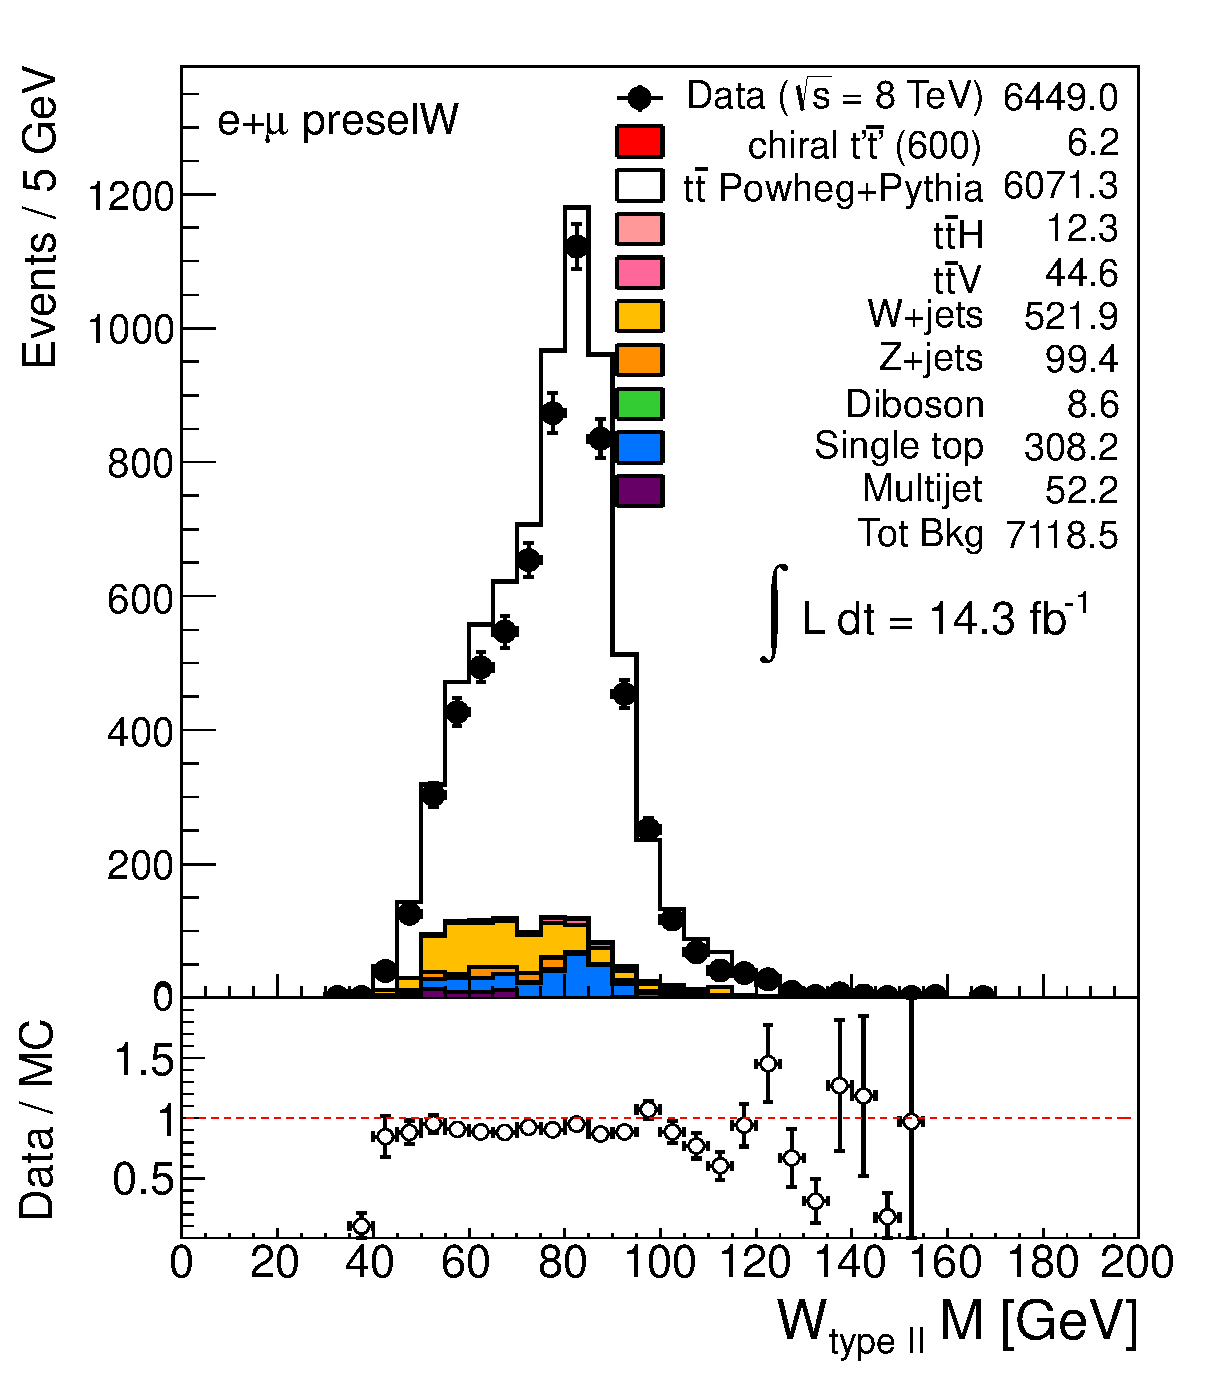
\includegraphics[width=1.\textwidth]{pics/VLQAna_WbX_WpreselType2_M_ELEMUON_preselW_NOMINAL}

\begin{pgfpicture}{0.0\textwidth}{0.0\textheight}{1.\textwidth}{.01\textwidth}
\begin{pgfscope}
 \pgfsetlinewidth{1.pt}
 \usebeamercolor[bg]{head/foot boxes}
 \pgfrect[stroke]{\pgfxy(1.85,0.85)}{\pgfxy(1.3,3.1)}
\end{pgfscope}
\end{pgfpicture}


\end{minipage}

\end{frame}

%%%%%%%%%%%%%%%%%%%%%%%%%
%%%
%%%%%%%%%%%%%%%%%%%%%%%%%
\begin{frame}\frametitle{Mass reconstruction}
\centering
\footnotesize


\begin{minipage}{.55\textwidth}

{
\centering

{\cccolor \wlep\ } reconstructed using {\cccolor lepton} and {\cccolor ``neutrino''}:\\
$p_X, p_Y$ from \met, $p_Z$ from $M_W^2 = (P_l + P_{\nu})^2$\\
{\large$\Downarrow$}\\
{\it two} possible solutions\\
}

\hspace{.75\textwidth}{\large$\searrow$}

\end{minipage}\begin{minipage}{.45\textwidth}

{
\centering

\myskip
one \bjet\ requested, two \bjet s needed\\
{\large$\Downarrow$}\\
consider the two jets with highest \btag-weight\\
}

{\large$\swarrow$}\\

\end{minipage}

\vskip-1ex
Pair \bjet s and $W$ boson candidates in order to get min$\Delta(M_{\rm lep},M_{\rm had})$\\
{\large$\Downarrow$}\\
%Discriminating variable: {\cccolor $T$ reconstructed mass}\\
%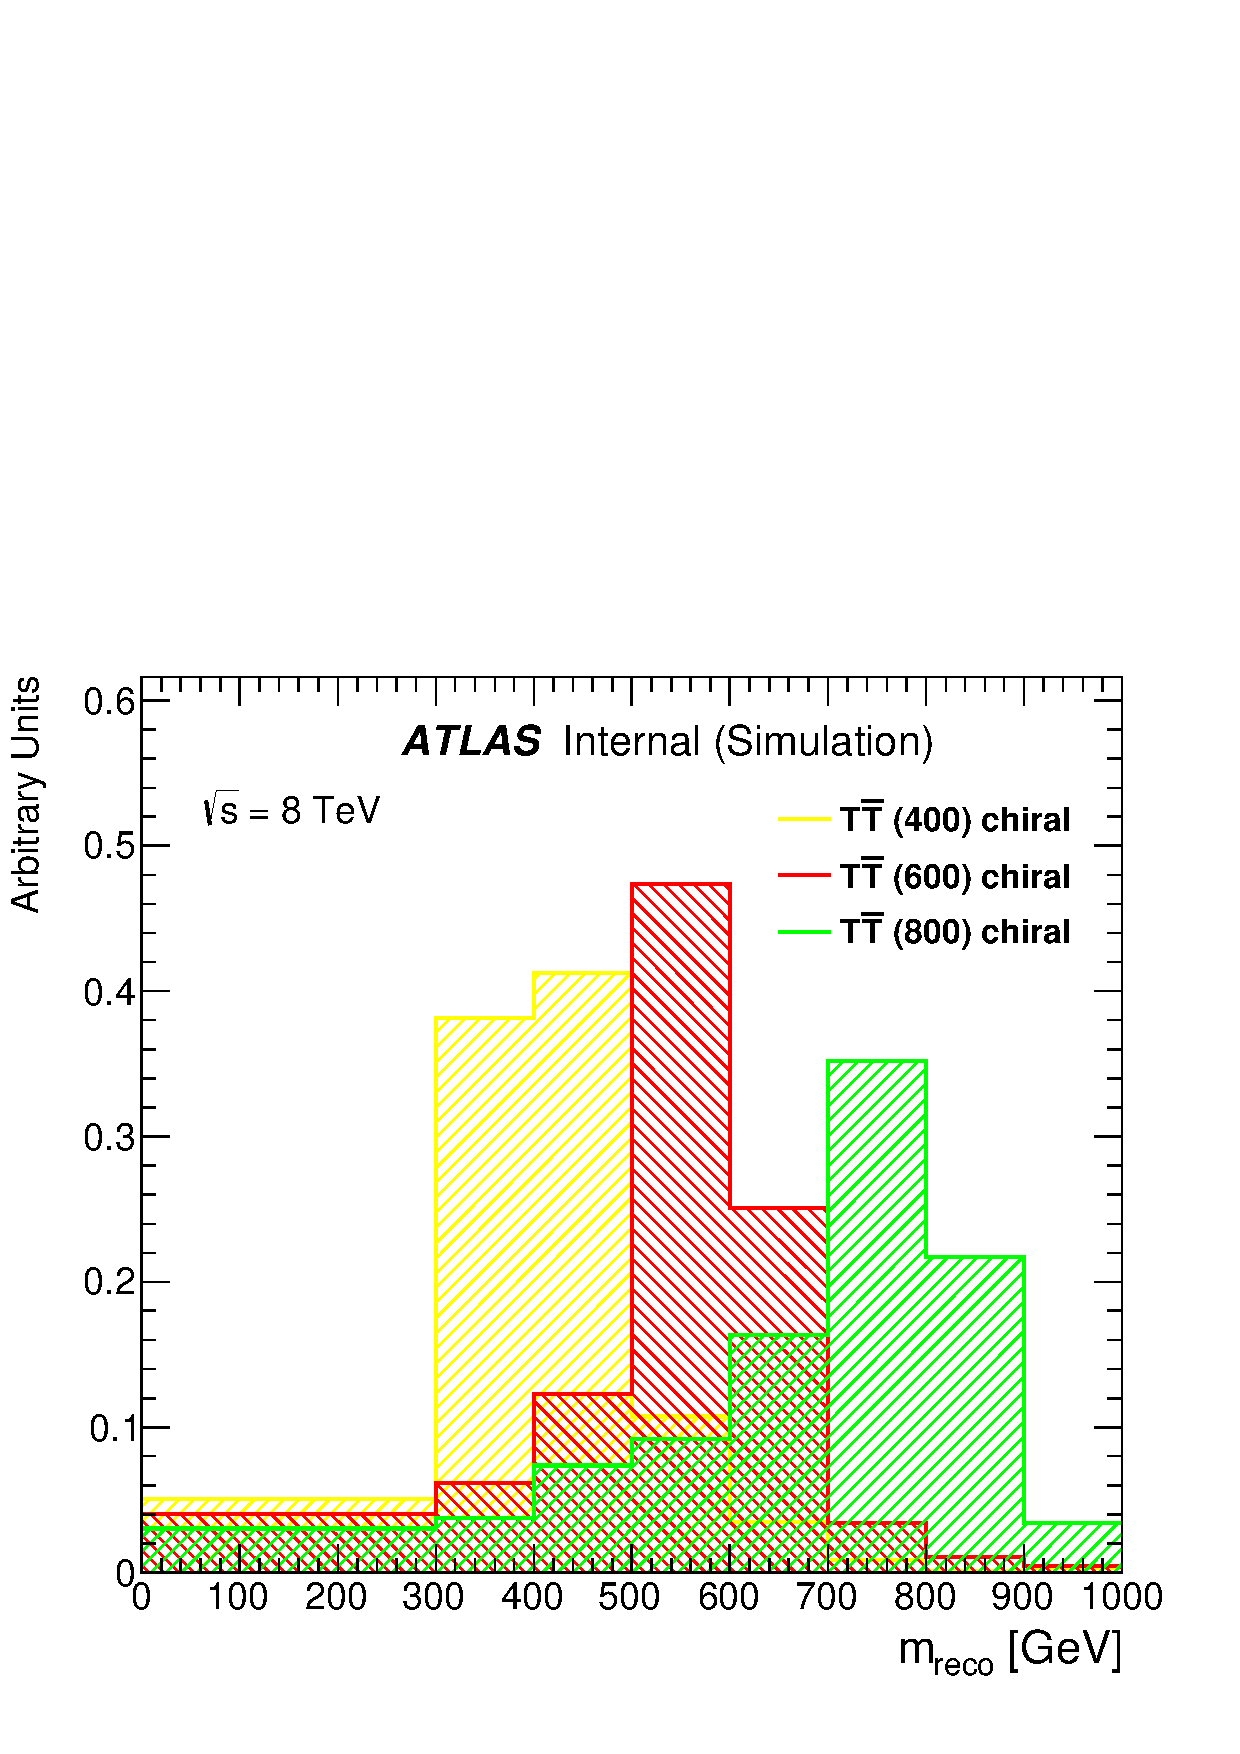
\includegraphics[width=.8\textwidth]{pics/VLQAna_WbX_1W_MWb_4_ELEMUONloose_1W_NOMINAL_VLTtt.pdf}\\
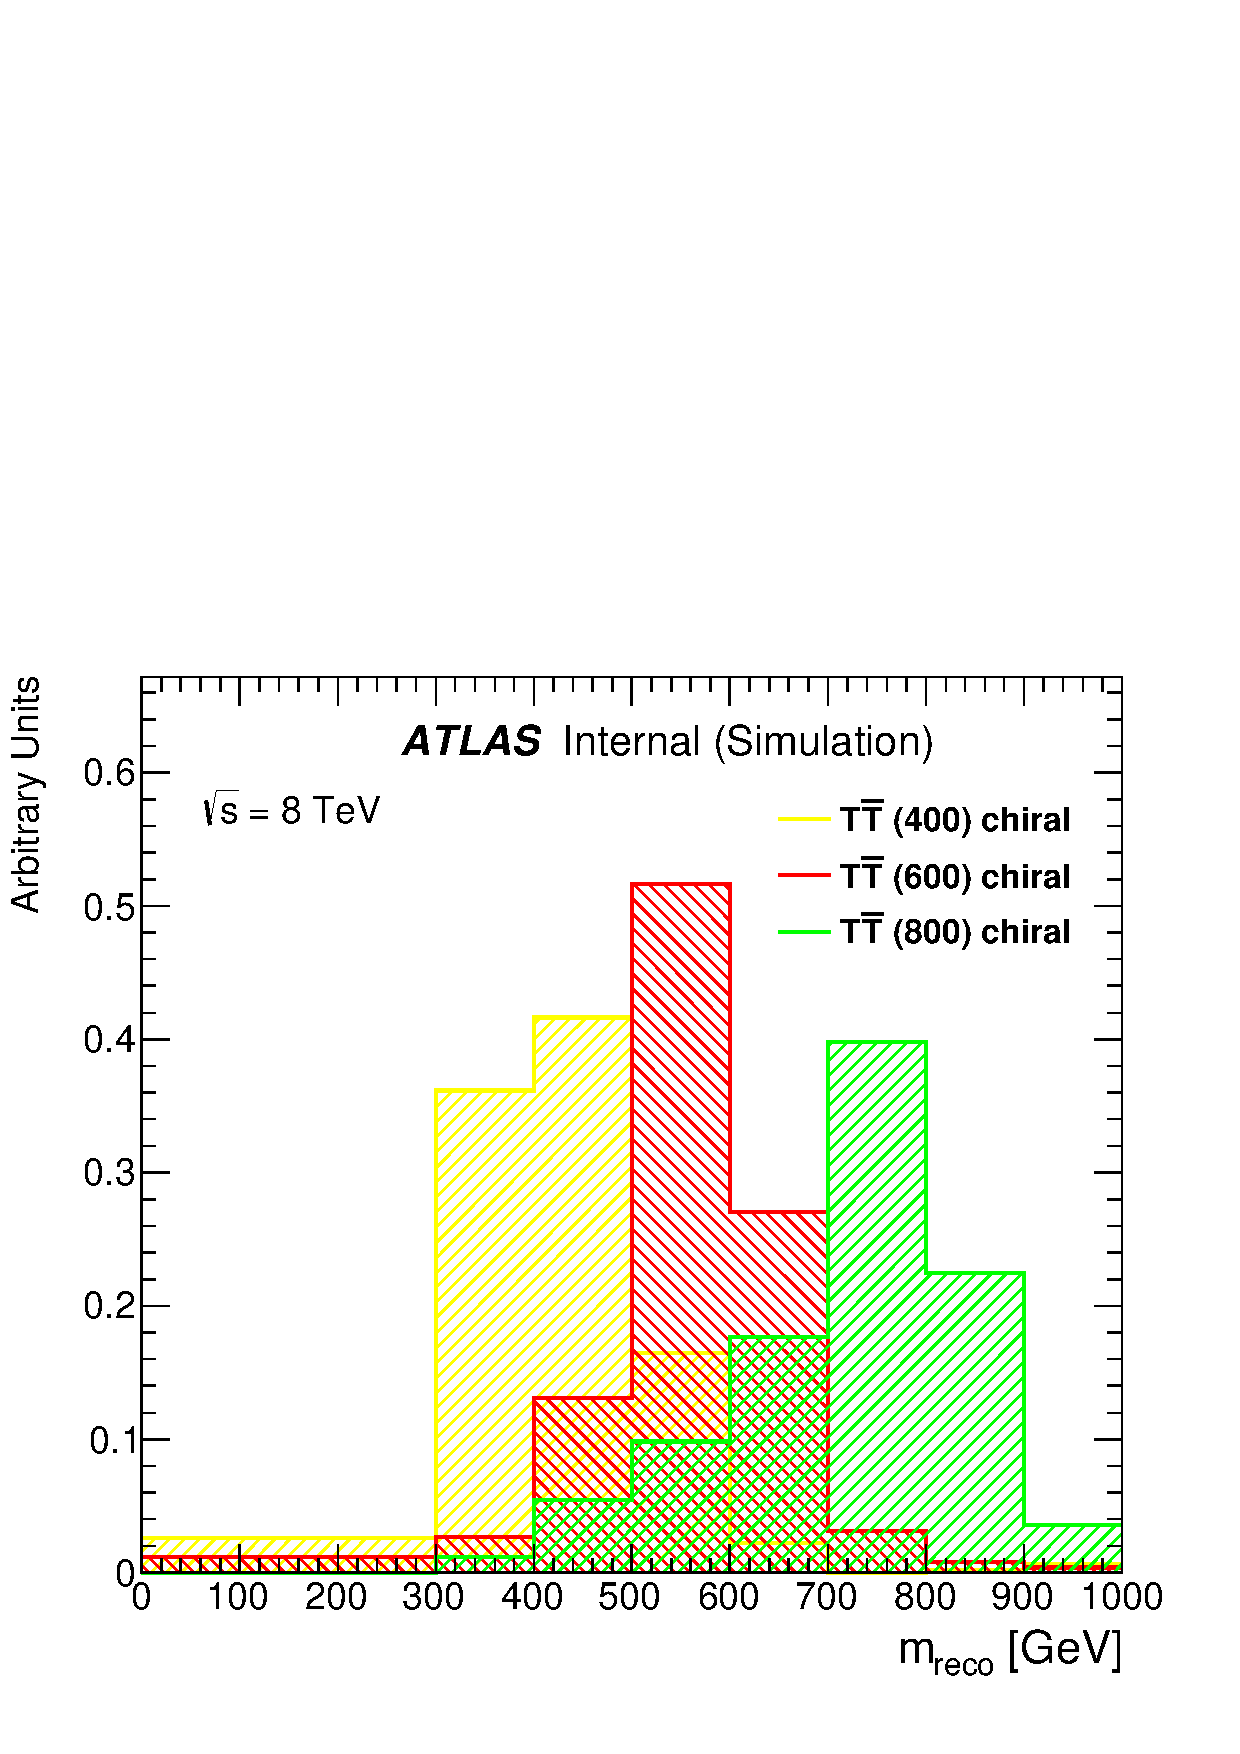
\includegraphics[width=.4\textwidth]{pics/VLQAna_WbX_1W_MWb_4_ELEMUONtight_1W_NOMINAL_VLTtt.pdf}

\end{frame}





%%%%%%%%%%%%%%%%%%%%%%%%%
%%%
%%%%%%%%%%%%%%%%%%%%%%%%%
\begin{frame}\frametitle{Event selection}
\centering\footnotesize

\begin{minipage}{.5\textwidth}\centering
\begin{tabular}{ll}
\toprule
\multicolumn{2}{c}{\loose\ selection}\\
 SR0 & Preselection + Ortho Cut (*) \\
 SR1 & +\hskip5ex$\geq 1~W_{\rm had}$ candidates \\
 SR2 & +\hskip5ex$\htfj>800\gev$ \\
 SR3 & +\hskip5ex $\pt(b_1) > 160\gev$\\
 SR4 & +\hskip5ex$\pt(b_2) >80\gev$ \\
 SR5 & +\hskip5ex$\Delta R(\ell,\nu)<1.2$ \\
\bottomrule
\toprule
\multicolumn{2}{c}{\tight\  selection} \\
 SR5 & \loose\ selection \\
 SR6 &  +\hskip5ex min$\Delta R(\ell,b)>1.4$\\
 SR7 & +\hskip5ex min$\Delta R(W_{\rm had},b)>1.4$ \\
\bottomrule
\end{tabular}

%N.B. \bjet s are the two jets with highest \btag\ weight

\end{minipage}\begin{minipage}{.5\textwidth}\centering



\begin{pgfpicture}{0.0\textwidth}{0.0\textheight}{1.\textwidth}{.6\textwidth}
   \begin{pgftranslate}{\pgfpoint{0.05\textwidth}{-0.12\textheight}}
\pgfdeclareimage[interpolate=true,width=.95\textwidth]{htall}{pics/HTAll_ELEMUON_cutflow1_NOMINAL.pdf}
\pgfdeclareimage[interpolate=true,width=.95\textwidth]{jetptb1}{pics/JetPtB1_ELEMUON_cutflow12_NOMINAL.pdf}
\pgfdeclareimage[interpolate=true,width=.95\textwidth]{jetptb2}{pics/JetPtB2_ELEMUON_cutflow123_NOMINAL.pdf}
\pgfdeclareimage[interpolate=true,width=.95\textwidth]{nwhad}{pics/nWhad_ELEMUON_cutflow0_NOMINAL_logscale.pdf}
\pgfdeclareimage[interpolate=true,width=.95\textwidth]{mrecoT}{pics/VLQAna_WbX_1W_MWb_4_ELEMUON_cutflow1234567_NOMINAL.pdf}
\pgfdeclareimage[interpolate=true,width=.95\textwidth]{mrecoL}{pics/VLQAna_WbX_1W_MWb_4_ELEMUON_cutflow12345_NOMINAL.pdf}
\pgfdeclareimage[interpolate=true,width=.95\textwidth]{drlep}{pics/VLQAna_WbX_DRLepMet_ELEMUON_cutflow1234_NOMINAL.pdf}
\pgfdeclareimage[interpolate=true,width=.95\textwidth]{mindrl}{pics/VLQAna_WbX_MinDRlb_ELEMUON_cutflow12345_NOMINAL.pdf}
\pgfdeclareimage[interpolate=true,width=.95\textwidth]{mindrw}{pics/VLQAna_WbX_MinDRWb_ELEMUON_cutflow123456_NOMINAL.pdf}
%\pgfputat{\pgfxy(0.0,0.0)}{\pgfbox[left,base]{\pgfuseimage{mindr}}}
\pgfputat{\pgfxy(-6.5,0.0)}{\pgfbox[left,base]{(*) reject events with $\geq$6 jets and $\geq$3 \bjet s}}
 \pgfsetlinewidth{1.pt}
 \usebeamercolor[bg]{head/foot boxes}
\only<1>{
 \pgfrect[stroke]{\pgfxy(-6,3.82)}{\pgfxy(5,0.35)}
 \pgfstroke
\pgfputat{\pgfxy(0.0,-0.8)}{\pgfbox[left,base]{\pgfuseimage{nwhad}}}
 {\usebeamercolor[fg]{head/foot boxes}
 \pgfline{\pgfxy(1.8,0.)}{\pgfxy(1.8,5.5)} }
}
\only<2>{
% \pgfrect[stroke]{\pgfxy(-6,3.46)}{\pgfxy(5,0.35)}
 \pgfrect[stroke]{\pgfxy(-6,2.74)}{\pgfxy(5,1.05)}
 %\pgfline{\pgfxy(1.55,1.5)}{\pgfxy(1.55,3.5)} 
 \pgfstroke
\pgfputat{\pgfxy(0.0,-0.8)}{\pgfbox[left,base]{\pgfuseimage{htall}}}
 {\usebeamercolor[fg]{head/foot boxes}
 \pgfline{\pgfxy(2.72,0.)}{\pgfxy(2.72,5.5)} }
}
\only<3>{
 \pgfrect[stroke]{\pgfxy(-6,2.45)}{\pgfxy(5,0.35)}
 %\pgfline{\pgfxy(1.55,1.5)}{\pgfxy(1.55,3.5)} 
 \pgfstroke
\pgfputat{\pgfxy(0.0,-0.8)}{\pgfbox[left,base]{\pgfuseimage{drlep}}}
 {\usebeamercolor[fg]{head/foot boxes}
 \pgfline{\pgfxy(2.4,0.)}{\pgfxy(2.4,5.5)} }
}
\only<4>{
 \pgfrect[stroke]{\pgfxy(-6,1.15)}{\pgfxy(5,0.35)}
 %\pgfline{\pgfxy(1.55,1.5)}{\pgfxy(1.55,3.5)} 
 \pgfstroke
\pgfputat{\pgfxy(0.0,-0.8)}{\pgfbox[left,base]{\pgfuseimage{mindrl}}}
 {\usebeamercolor[fg]{head/foot boxes}
 \pgfline{\pgfxy(2.7,0.)}{\pgfxy(2.7,5.5)} }
}
\only<5>{
 \pgfrect[stroke]{\pgfxy(-6,0.8)}{\pgfxy(5,0.35)}
 %\pgfline{\pgfxy(1.55,1.5)}{\pgfxy(1.55,3.5)} 
 \pgfstroke
\pgfputat{\pgfxy(0.0,-0.8)}{\pgfbox[left,base]{\pgfuseimage{mindrw}}}
 {\usebeamercolor[fg]{head/foot boxes}
 \pgfline{\pgfxy(2.7,0.)}{\pgfxy(2.7,5.5)} }
}
   \end{pgftranslate}

\end{pgfpicture}

\end{minipage}

\end{frame}


%%%%%%%%%%%%%%%%%%%%%%%%%
%%%
%%%%%%%%%%%%%%%%%%%%%%%%%
\begin{frame}\frametitle{Comparison data vs prediction}
\centering\footnotesize

\begin{minipage}{.5\textwidth}\centering

Check agreement between data and background prediction

{\Large$\Downarrow$}

Define regions depleted in signal

\myskip

\scriptsize
\begin{tabular}{l*{1}{r@{ $\pm$ }r@{ }l}}
\toprule
 & \multicolumn{3}{c}{\loose\ but $\Delta R(\ell,\nu)>1.2$}\\
\midrule
$t\bar{t'} (600\GeV)$ & $18.47$ & $1.48$ & $^{+1.09}_{-1.64}$\\
\midrule
$t\bar{t}$ & $173.13$ & $8.82$ & $^{+46.92}_{-48.59}$\\
$W$+jets & $30.64$ & $9.78$ & $^{+13.74}_{-12.43}$\\
$Z$+jets & $11.68$ & $5.93$ & $^{+5.89}_{-6.96}$\\
Diboson & $0.29$ & $0.19$ & $^{+0.17}_{-0.17}$\\
Single top & $21.46$ & $2.54$ & $^{+2.60}_{-2.54}$\\
$t\bar{t}$$V$ & $4.21$ & $0.16$ & $^{+1.33}_{-1.33}$\\
Multijet & $0.49$ & $0.91$ & $ \pm\ 0.25$\\
\midrule
Total bkg. & $241.90 $ & $ 14.70$ & $ ^{+53.57}_{-55.95}$\\
\midrule
Data & \multicolumn{3}{c}{$250$}\\
\bottomrule
\end{tabular}


\end{minipage}\begin{minipage}{.5\textwidth}\centering

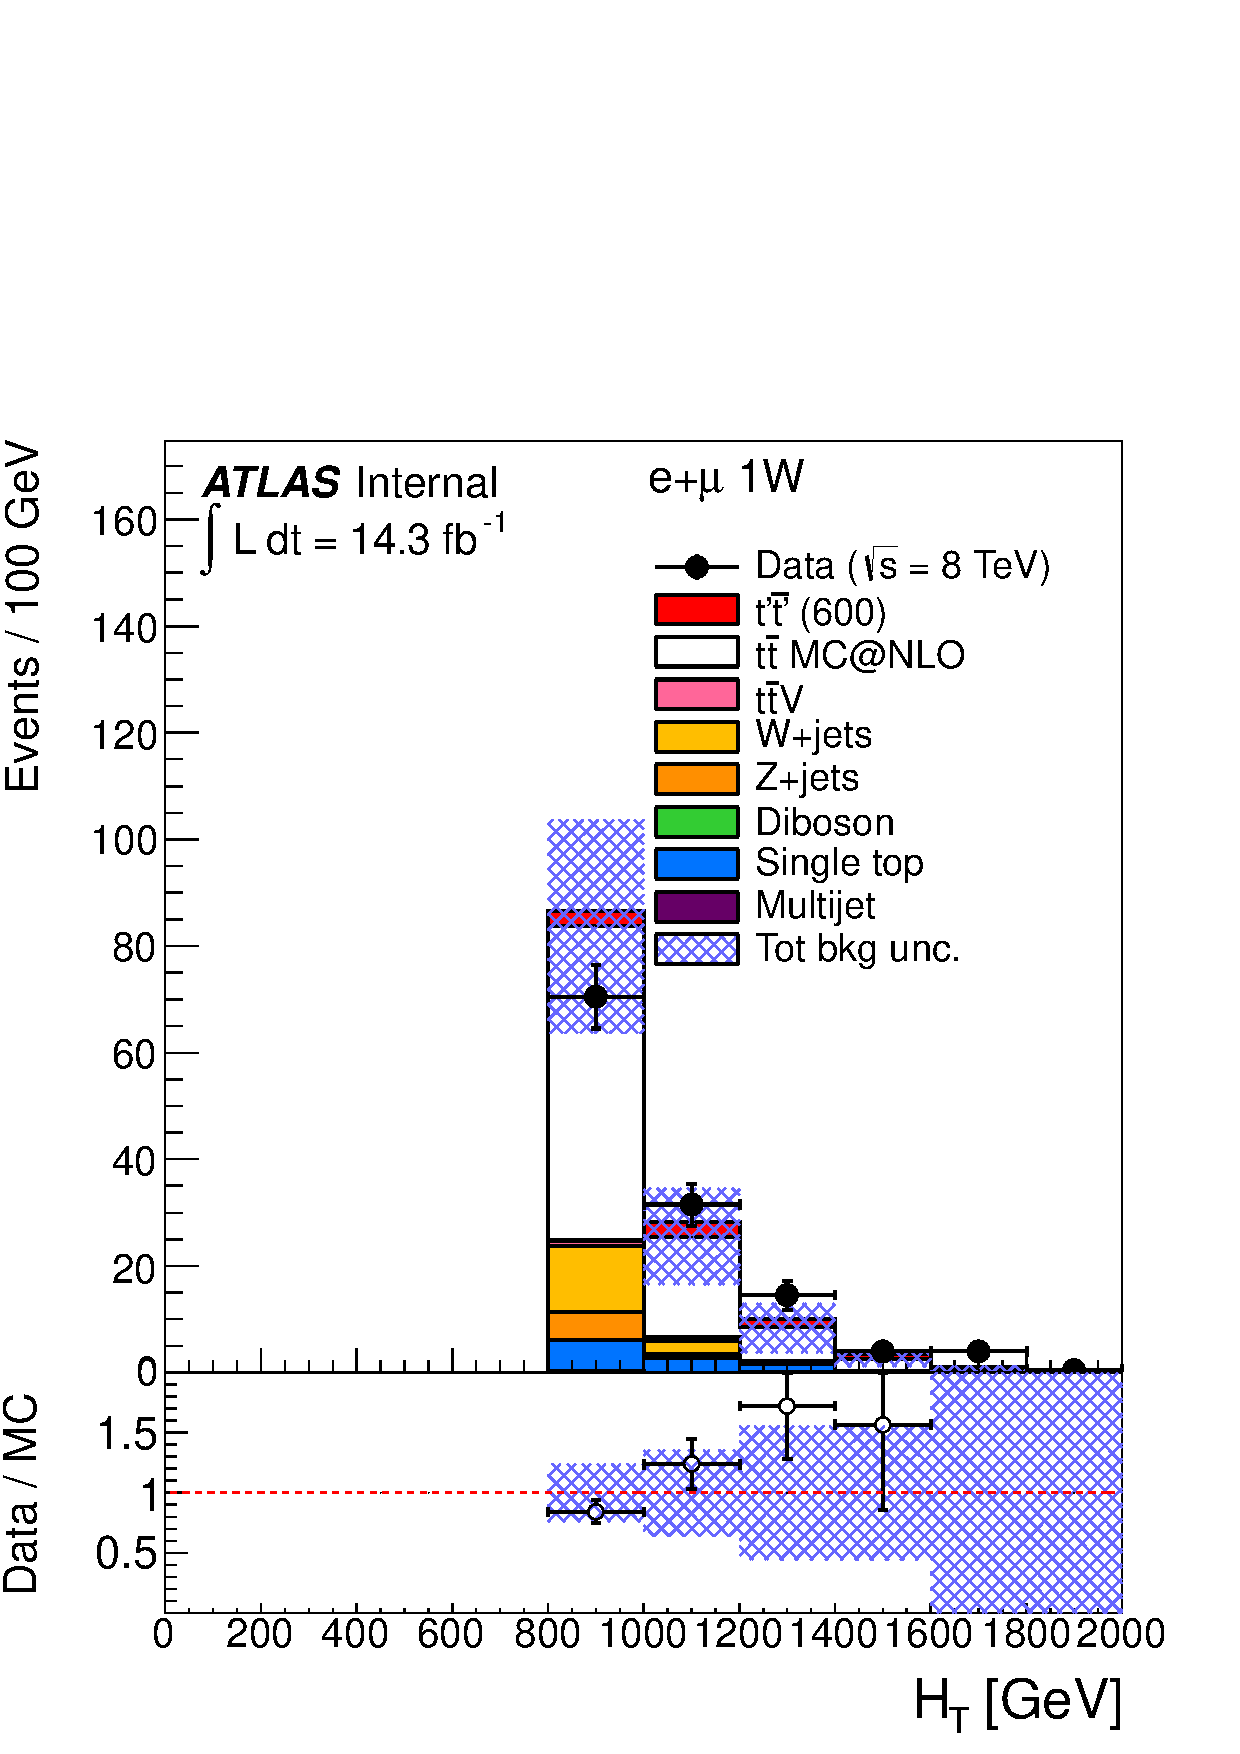
\includegraphics[width=.5\textwidth]{pics/HTAll_ELEMUONCR3_1W_NOMINAL.pdf}
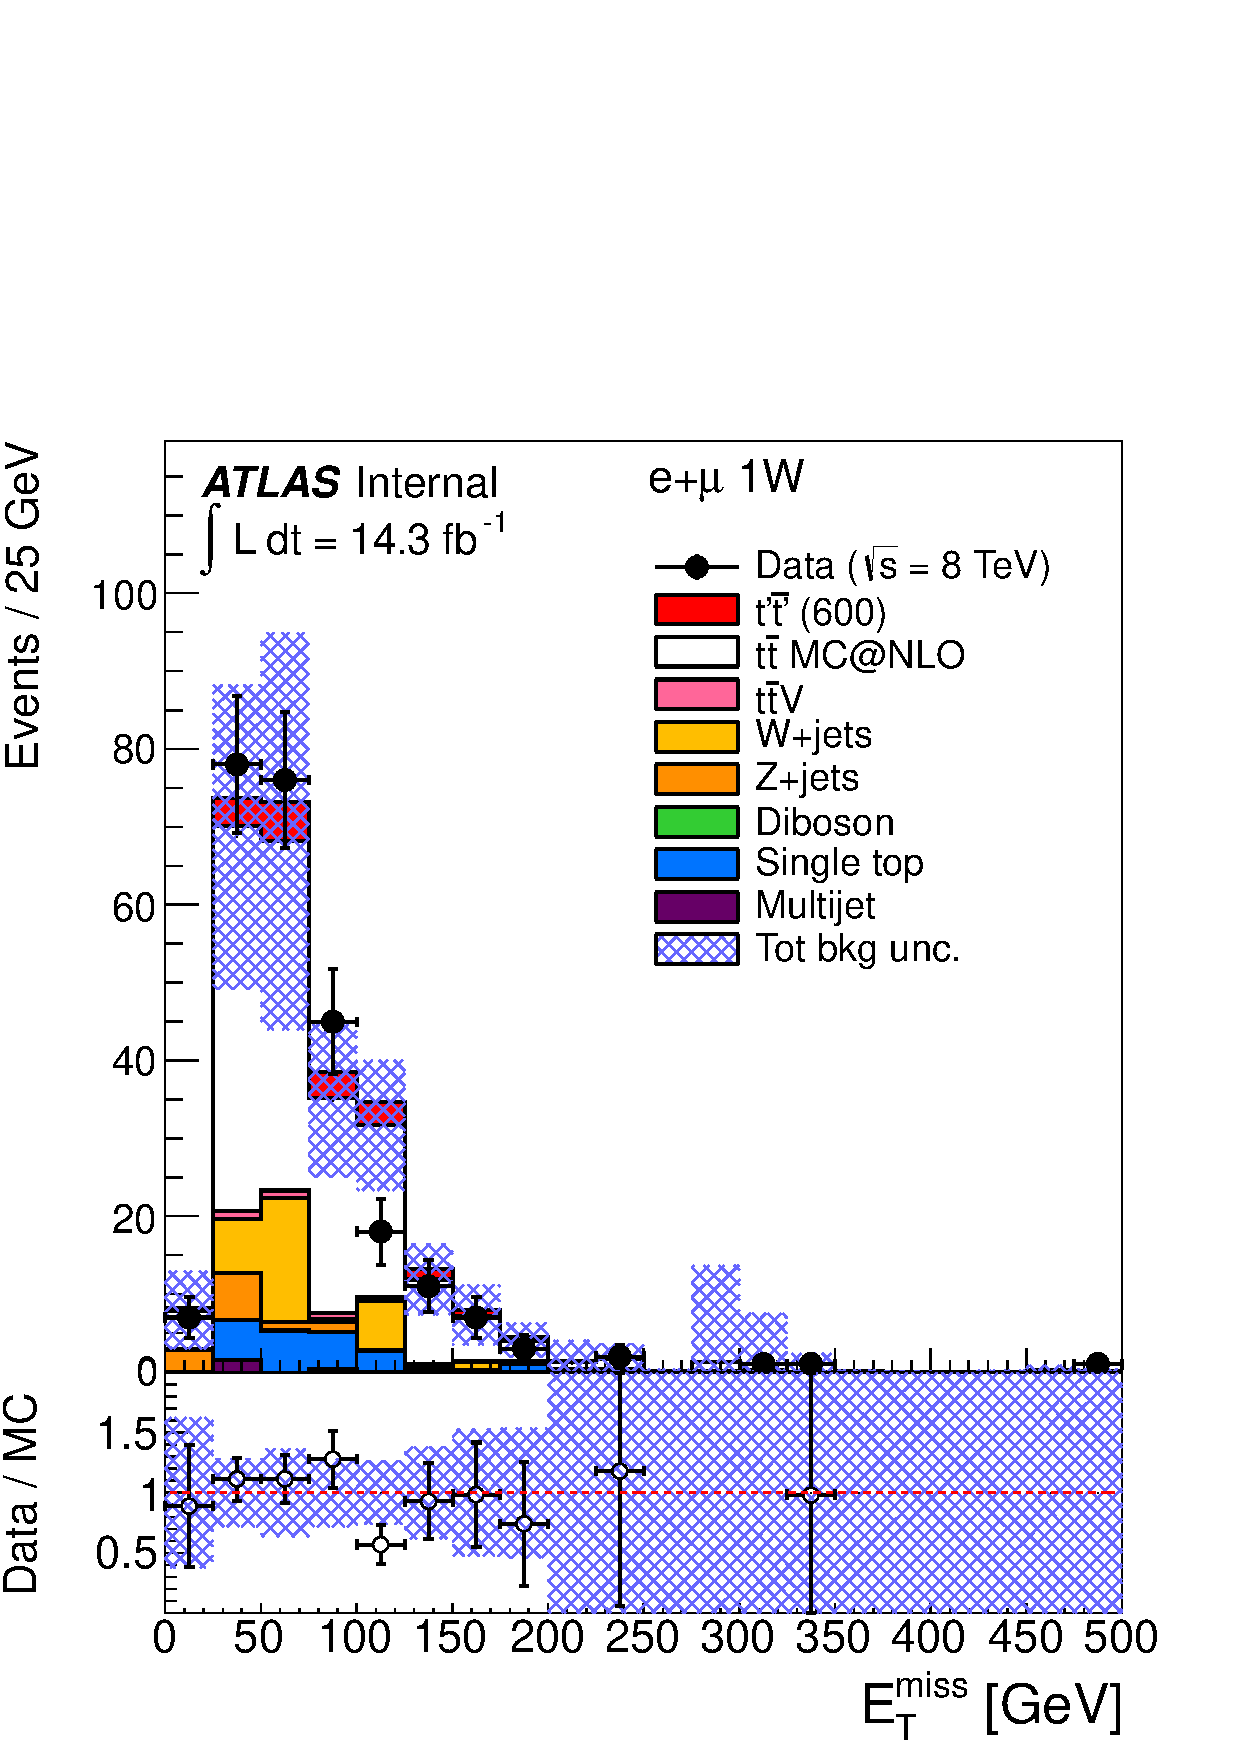
\includegraphics[width=.5\textwidth]{pics/MET_ELEMUONCR3_1W_NOMINAL.pdf}\\
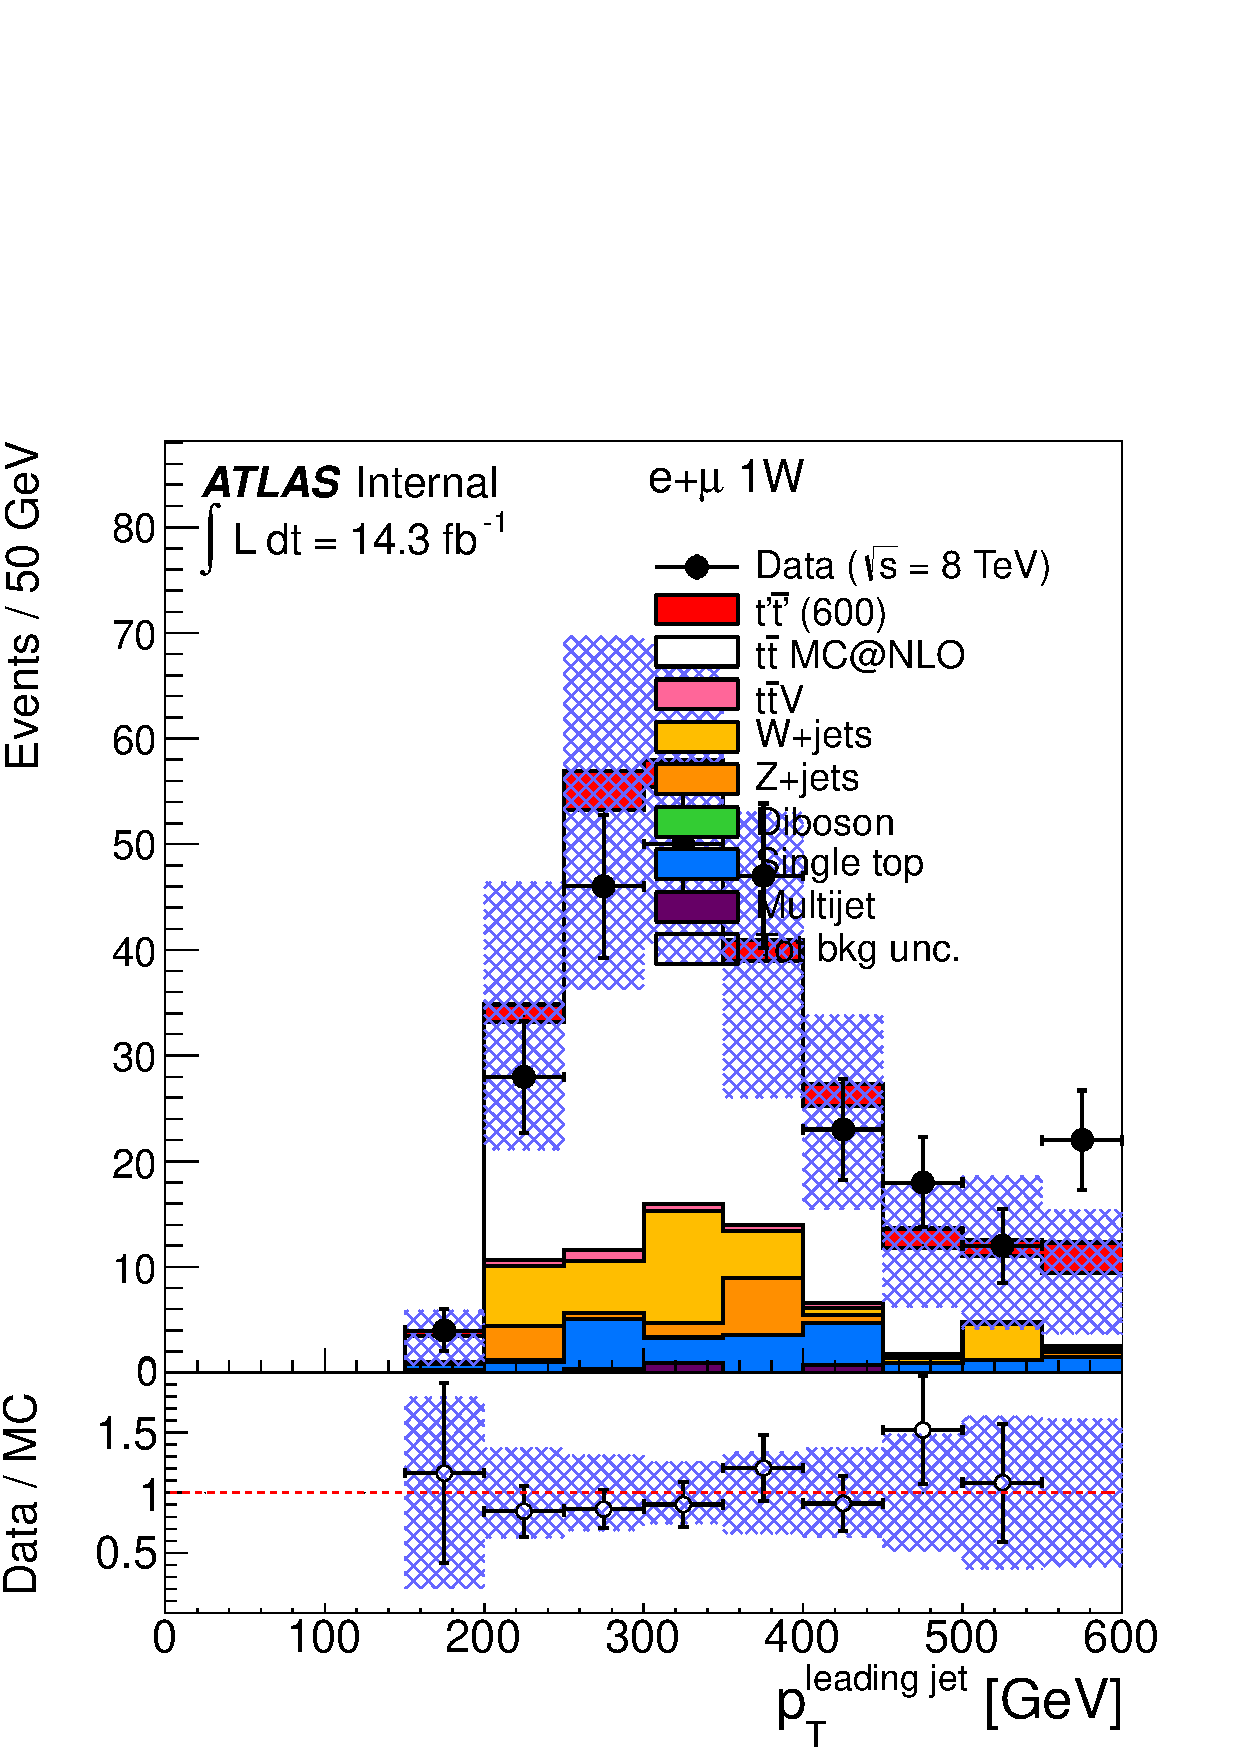
\includegraphics[width=.5\textwidth]{pics/JetPt1_ELEMUONCR3_1W_NOMINAL.pdf}
\includegraphics[width=.5\textwidth]{pics/Njets25_ELEMUONCR3_1W_NOMINAL.pdf}

\end{minipage}

\end{frame}


%%%%%%%%%%%%%%%%%%%%%%%%%
%%%
%%%%%%%%%%%%%%%%%%%%%%%%%
\begin{frame}\frametitle{Final discriminant}
\centering\footnotesize

\begin{minipage}{.5\textwidth}\centering

\begin{tabular}{ll}
\toprule
\multicolumn{2}{c}{\loose\ selection}\\
 SR0 & Preselection  \\
 SR1 & +\hskip5ex$\geq 1~W_{\rm had}$ candidates \\
 SR2 & +\hskip5ex$\htfj>800\gev$ \\
 SR3 & +\hskip5ex $\pt(b_1) > 160\gev$\\
 SR4 & +\hskip5ex$\pt(b_2) >80\gev$ \\
 SR5 & +\hskip5ex$\Delta R(\ell,\nu)<1.2$ \\
\bottomrule
\toprule
\multicolumn{2}{c}{\tight\  selection} \\
 SR5 & \loose\ selection \\
 SR6 &  +\hskip5ex min$\Delta R(\ell,b)>1.4$\\
 SR7 & +\hskip5ex min$\Delta R(W_{\rm had},b)>1.4$ \\
\bottomrule
\end{tabular}
%N.B. \bjet s are the two jets with highest \btag\ weight

\end{minipage}\begin{minipage}{.5\textwidth}\centering



\begin{pgfpicture}{0.0\textwidth}{0.0\textheight}{1.\textwidth}{.6\textwidth}
   \begin{pgftranslate}{\pgfpoint{0.05\textwidth}{-0.12\textheight}}

\pgfdeclareimage[interpolate=true,width=.95\textwidth]{mreco6}{pics/THESIS_c6_cutflow/VLQAna_WbX_1W_MWb_4_ELEMUON_cutflow123456_NOMINAL.pdf}
\pgfdeclareimage[interpolate=true,width=.95\textwidth]{mreco4}{pics/THESIS_c6_cutflow/VLQAna_WbX_1W_MWb_4_ELEMUON_cutflow1234_NOMINAL.pdf}
\pgfdeclareimage[interpolate=true,width=.95\textwidth]{mreco3}{pics/THESIS_c6_cutflow/VLQAna_WbX_1W_MWb_4_ELEMUON_cutflow123_NOMINAL.pdf}
\pgfdeclareimage[interpolate=true,width=.95\textwidth]{mreco2}{pics/THESIS_c6_cutflow/VLQAna_WbX_1W_MWb_4_ELEMUON_cutflow12_NOMINAL.pdf}
\pgfdeclareimage[interpolate=true,width=.95\textwidth]{mreco1}{pics/THESIS_c6_cutflow/VLQAna_WbX_1W_MWb_4_ELEMUON_cutflow1_NOMINAL.pdf}
\pgfdeclareimage[interpolate=true,width=.95\textwidth]{mrecoT}{pics/VLQAna_WbX_1W_MWb_4_ELEMUON_cutflow1234567_NOMINAL.pdf}
\pgfdeclareimage[interpolate=true,width=.95\textwidth]{mrecoL}{pics/VLQAna_WbX_1W_MWb_4_ELEMUON_cutflow12345_NOMINAL.pdf}
%\pgfputat{\pgfxy(0.0,0.0)}{\pgfbox[left,base]{\pgfuseimage{mindr}}}
 \pgfsetlinewidth{1.pt}
 \usebeamercolor[bg]{head/foot boxes}
\only<1>{
 \pgfrect[stroke]{\pgfxy(-6,3.82)}{\pgfxy(5,0.35)}
 %\pgfline{\pgfxy(1.55,1.5)}{\pgfxy(1.55,3.5)} 
 \pgfstroke
\pgfputat{\pgfxy(0.0,-0.8)}{\pgfbox[left,base]{\pgfuseimage{mreco1}}}
}
\only<2>{
 \pgfrect[stroke]{\pgfxy(-6,3.46)}{\pgfxy(5,0.35)}
 %\pgfline{\pgfxy(1.55,1.5)}{\pgfxy(1.55,3.5)} 
 \pgfstroke
\pgfputat{\pgfxy(0.0,-0.8)}{\pgfbox[left,base]{\pgfuseimage{mreco2}}}
}
\only<3>{
 \pgfrect[stroke]{\pgfxy(-6,3.1)}{\pgfxy(5,0.35)}
 %\pgfline{\pgfxy(1.55,1.5)}{\pgfxy(1.55,3.5)} 
 \pgfstroke
\pgfputat{\pgfxy(0.0,-0.8)}{\pgfbox[left,base]{\pgfuseimage{mreco3}}}
}
\only<4>{
 \pgfrect[stroke]{\pgfxy(-6,2.74)}{\pgfxy(5,0.35)}
 %\pgfline{\pgfxy(1.55,1.5)}{\pgfxy(1.55,3.5)} 
 \pgfstroke
\pgfputat{\pgfxy(0.0,-0.8)}{\pgfbox[left,base]{\pgfuseimage{mreco4}}}
}
\only<5>{
 \pgfrect[stroke]{\pgfxy(-6,2.45)}{\pgfxy(5,0.35)}
 %\pgfline{\pgfxy(1.55,1.5)}{\pgfxy(1.55,3.5)} 
 \pgfstroke
\pgfputat{\pgfxy(0.0,-0.8)}{\pgfbox[left,base]{\pgfuseimage{mrecoL}}}
}
\only<6>{
 \pgfrect[stroke]{\pgfxy(-6,1.15)}{\pgfxy(5,0.35)}
 %\pgfline{\pgfxy(1.55,1.5)}{\pgfxy(1.55,3.5)} 
 \pgfstroke
\pgfputat{\pgfxy(0.0,-0.8)}{\pgfbox[left,base]{\pgfuseimage{mreco6}}}
}
\only<7>{
 \pgfrect[stroke]{\pgfxy(-6,0.8)}{\pgfxy(5,0.35)}
 %\pgfline{\pgfxy(1.55,1.5)}{\pgfxy(1.55,3.5)} 
 \pgfstroke
\pgfputat{\pgfxy(0.0,-0.8)}{\pgfbox[left,base]{\pgfuseimage{mrecoT}}}
}
   \end{pgftranslate}

\end{pgfpicture}

\end{minipage}

\end{frame}


%%%%%%%%%%%%%%%%%%%%%%%%%
%%%
%%%%%%%%%%%%%%%%%%%%%%%%%
\begin{frame}\frametitle{Final discriminant}
\centering\footnotesize

\begin{minipage}{.5\textwidth}\centering

\begin{tabular}{p{0.05cm} p{0.05cm}}
\\
\\
%\parbox[t]{2mm}{\multirow{5}{*}{\rotatebox[origin=c]{90}{rota}}}& \ldelim\{{5}{5ex} \\
\multirow{5}{*}{\rotatebox[origin=c]{90}{\cccolor merged}}& \ldelim\{{5}{5ex} \\
\\
\\
\\
\\
\\
\\
\\
\\
\\
\\
\end{tabular}\begin{tabular}{l  D{;}{\,\pm\,}{-1} }
    \toprule
    & \multicolumn{1}{c}{\tight}  \\\midrule
$t\bar{t}$    & 10;6 \\
$t\bar{t}V$   & 0.5;0.2 \\
$W$+jets   &  6;5\\
$Z$+jets   &  0.2;0.5 \\
Single top   & 4.4;1.6  \\
Dibosons & 0.06;0.05 \\
\midrule
Tot.Bkg.  & 21;9 \\
Data & 37  \\
%Data& \multicolumn{1}{c}{348\,\phantom{$\pm$}} & 37  \\
\midrule
$T\bar{T}(600\GeV)$ \\
Chiral $t'$&  54;7 \\
$T$ Singlet  & 20.3;2.2 \\
\bottomrule\end{tabular}


\end{minipage}\begin{minipage}{.5\textwidth}\centering



\begin{pgfpicture}{0.0\textwidth}{0.0\textheight}{1.\textwidth}{.6\textwidth}
   \begin{pgftranslate}{\pgfpoint{0.05\textwidth}{-0.12\textheight}}
\pgfdeclareimage[interpolate=true,width=.95\textwidth]{mrecoT}{pics/VLQAna_WbX_1W_MWb_4_ELEMUON_cutflow1234567_NOMINAL.pdf}
%\pgfputat{\pgfxy(0.0,0.0)}{\pgfbox[left,base]{\pgfuseimage{mindr}}}
 \pgfsetlinewidth{1.pt}
 \usebeamercolor[bg]{head/foot boxes}
 \pgfputat{\pgfxy(0.0,-0.8)}{\pgfbox[left,base]{\pgfuseimage{mrecoT}}}
   \end{pgftranslate}

\end{pgfpicture}

\end{minipage}

\end{frame}


%%%%%%%%%%%%%%%%%%%%%%%%%
%%%
%%%%%%%%%%%%%%%%%%%%%%%%%
\begin{frame}\frametitle{Most relevant systematic uncertainties}
\centering\footnotesize

\ttbar\ modeling systematics:
\begin{itemize}
\item Generator: \texttt{MC@NLO} vs \texttt{POWHEG}, both interfaced with \texttt{HERWIG}
\item Parton shower and fragmentation: same parton level generator (\texttt{POWHEG}) different hadronization models (\texttt{HERWIG}, \texttt{PYTHIA})
\item Initial- and final-state radiation: dedicated \texttt{ACERMC+PYTHIA} samples with varied parameters
\end{itemize}

\begin{tabular}{l*{3}{c}}
\toprule
 & $\T\bar{\T}$ ($600\gev$) & $t\bar{t}$ & Non-$t\bar{t}$\\
\midrule
Total [\%] & +14/-15 & +59/-59 & +42/-35\\
\midrule
Main contributions [\%] &&&\\
Jet energy scale & +6.6/-8.4 & +15/-15 & +33/-22\\  
$t\bar{t}$ modelling: NLO MC generator & -- & +48/-48 & --\\  
$t\bar{t}$ modelling: PS and fragm & -- & +25/-25 & --\\  
$t\bar{t}$ modelling: ISR/FSR & -- & +8.8/-8.8 & --\\   
\bottomrule
\end{tabular}

\end{frame}


\begin{frame}\frametitle{Statistical analysis}
\centering\myskip\scriptsize


\begin{minipage}{.5\textwidth}\centering

\cls{s}\ method~\cite{cls,cls_2}:

\begin{itemize}
\item ``background only'' hypothesis $\mathcal{H}_{b}$
\item ``signal plus background'' hypothesis $\mathcal{H}_{s+b}$ 
\item test statistic $Q$
\item $Q_{\rm obs} = $ observed value
\end{itemize}

\vskip-5ex
\begin{eqnarray*}
\cls{b} &=& P(Q \leq Q_{\rm obs}|\mathcal{H}_{b})\\
\cls{s+b} &=& P(Q \leq Q_{\rm obs}|\mathcal{H}_{s+b})\\
\cls{s} &=& \cls{s+b}/\cls{b}
\end{eqnarray*}

\footnotesize
{\cccolor Exclude} signal hypothesis at $\geq$ 95\% CL if $\cls{s} \leq 0.05$ 

\end{minipage}\begin{minipage}{.5\textwidth}\centering

Test statistic: Log-Likelihood Ratio

$$LLR = -2\log \dfrac{\mathcal{L}({\rm data}|\mathcal{H}_{s+b})}{\mathcal{L}({\rm data}|\mathcal{H}_{b})}$$

with $\mathcal{L}$ binned likelihoods from discriminating variable distribution

\includegraphics[width=0.9\textwidth]{pics/LLRtight_500GeV_stat}

\end{minipage}


%$\cls{s} < 0.05$ are deemed to be excluded at the 95\% CL.
%Using $\cls{s}$ instead of $\cls{s+b}$ minimizes the possibility  of mistakenly excluding a small signal due to a downward background fluctuation, as this would lead to small values of both $\cls{s+b}$ and $\cls{b}$.

%Similarly, the confidence level for excluding the background only hypothesis is the $p$-value $1 - \cls{b}$ and the value required to claim discovery is of $\sim 10^{-7}$. The motivation that led to the definition of \cls{s} instead of using \cls{s+b}, which also corresponds to the confidence level in excluding the signal+background hypothesis, is that the latter might wrongly exclude scenarios to which the analysis is simply non-sensitive to like is the general case for searches for rare events.


\end{frame}

%%%%%%%%%%%%%%%%%%%%%%%%%
%%%
%%%%%%%%%%%%%%%%%%%%%%%%%
\begin{frame}\frametitle{Benchmark results}
\centering\footnotesize

\begin{minipage}{.5\textwidth}\centering

Chiral \T/Vector-like $Y(-4/3)$\\

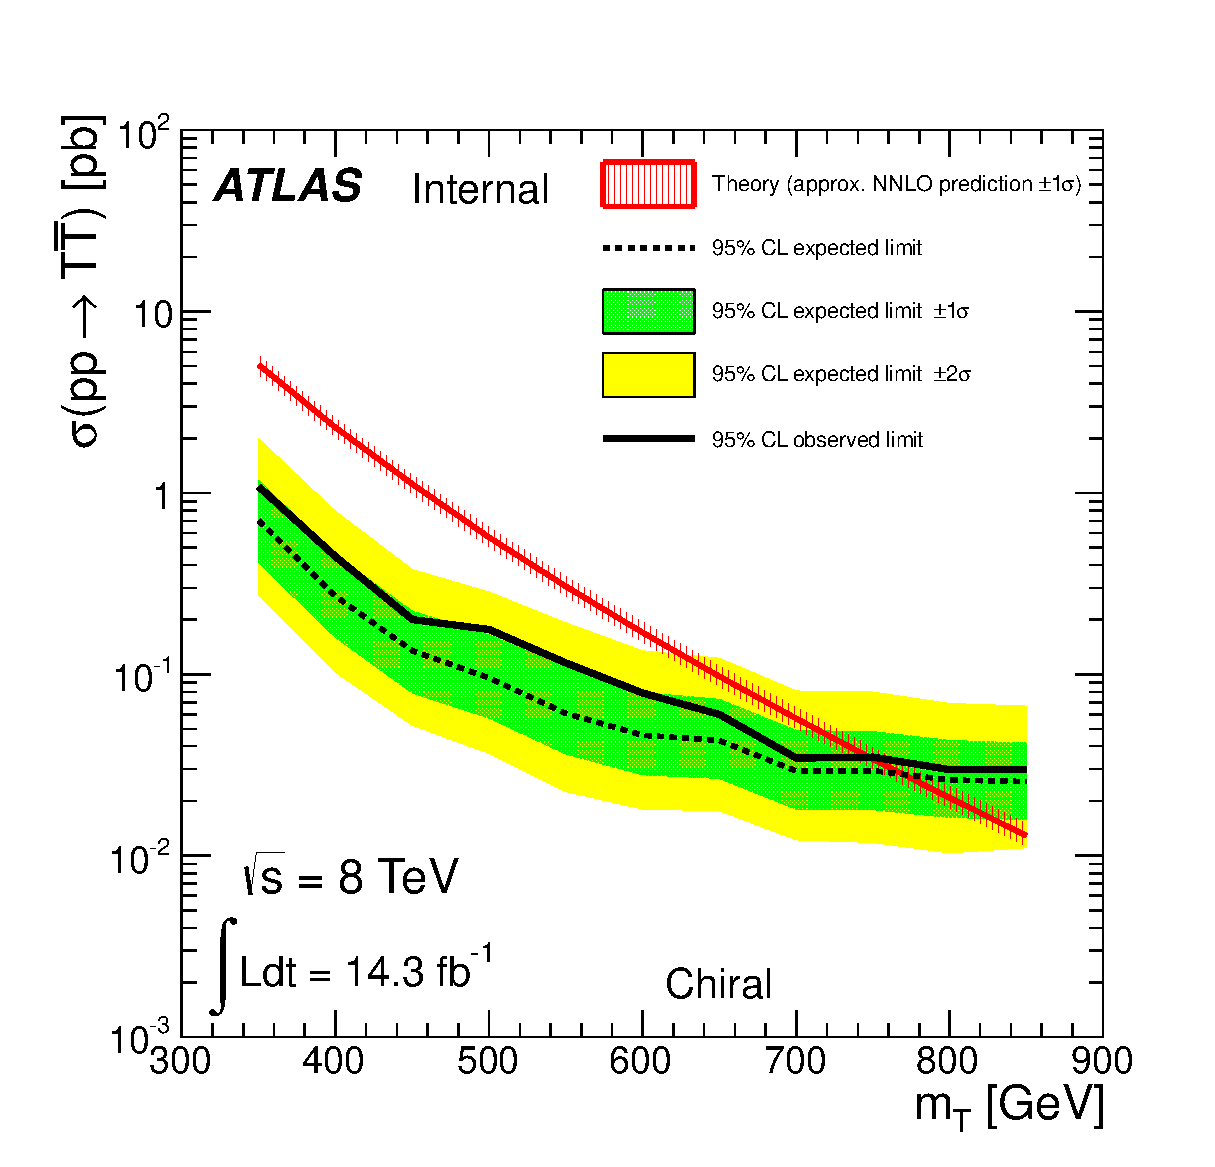
\includegraphics[width=0.9\textwidth]{pics/lim_chiral_bin1_WbX}\\

observed (expected) 95\%  CL limit $m_{\T}>740\,(770)\gev$

\end{minipage}\begin{minipage}{.5\textwidth}\centering

Singlet \T\\

\includegraphics[width=0.9\textwidth]{pics/lim_singlet_bin1_WbX}\\

observed (expected) 95\%  CL  limit 
$m_{\T}>505\,(630)\gev$ 

\end{minipage}


\end{frame}

%%%%%%%%%%%%%%%%%%%%%%%%%
%%%
%%%%%%%%%%%%%%%%%%%%%%%%%
\begin{frame}\frametitle{Model independent results}
\centering\footnotesize

\includegraphics[width=0.7\textwidth]{pics/lim_Scan2D_tight_Bin1.pdf}

\end{frame}




